Find the steady state of the output signal $y(t)$ if both the reference $r(t)$ and the disturbance $d(t)$ are unit steps. There are several ways to approach this problem, but one way is to use the property of superposition.
\begin{center}
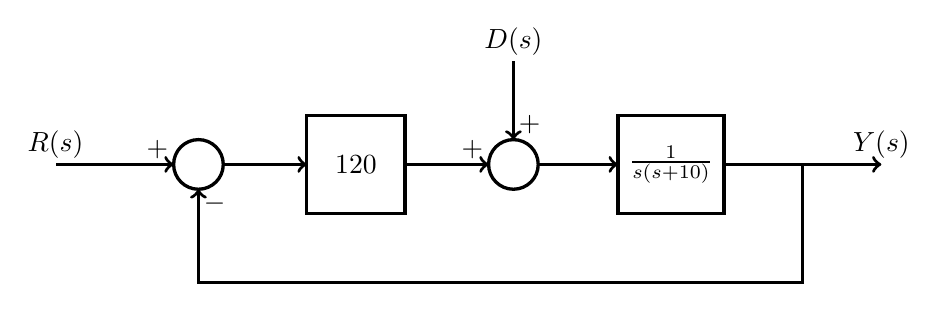
\begin{tikzpicture}[scale=1,inner sep=0pt,outer sep=0pt,very thick,
sysblock/.style={draw,rectangle,inner sep=4pt,minimum width=1.25cm,minimum height=1.25cm,very thick}]

\draw (-6,0) node[draw,circle] (sum1) {$\rule{0pt}{18pt}$};
\draw (-4,0) node[sysblock] (K) {120};
\draw (-2,0) node[draw,circle] (sum2) {$\rule{0pt}{18pt}$};
\draw (0,0) node[sysblock] (G) {$\frac{1}{s(s+10)}$};
\draw[<-] (sum1.180) node[above left=2pt] {$+$} -- ++(-1.5,0) node[above=2pt] {$R(s)$};
\draw[->] (sum1.0) -- (K.180);
\draw[->] (K.0) -- (sum2.180) node[above left=2pt] {$+$};
\draw[->] (sum2.0) -- (G.180);
\draw[<-] (sum2.90) node[above right=2pt] {$+$} -- ++(0,1) node[above=2pt] {$D(s)$};
\draw[->] (G.0) --  ++(2,0) node[above=2pt] {$Y(s)$};
\draw[->] (G.0) -- ++(1,0) -- ++(0,-1.5) -| (sum1.-90) node[below right=2pt] {$-$};
\end{tikzpicture}
\end{center}